%*******10********20********30********40********50********60********70********80

% For all chapters, use the newdefined chap{} instead of chapter{}
% This will make the text at the top-left of the page be the same as the chapter

\chap{AuthorVis: A Co-authorship Visualization and Scientific Collaboration Prediction tool}

\section{Background}
In this chapter, we propose a co-authorship network exploration, and link prediction tool specific to the three networks investigated in this dissertation. While many network visualization solutions have already been published, most of them are not specifically adapted to co-authorship network \cite{nakazono_nel_2006,odoni_visualisation_2017,liu_toolkits_2004,horak_forcoa.net:_2011}. 
% New citation to add: nakazono_nel_2006,odoni_visualisation_2017,liu_toolkits_2004,horak_forcoa.net:_2011,mena-chalco_brazilian_2014
Even those designed for visualizing co-authorship network have several limitations among others, their inability to satisfactorily display large networks, the lack of interactivity in the display, and the inability for the end user to control the display \cite{nakazono_nel_2006}.\\
Here, we present a tool that not only provides a visualization of each of the networks but allow the end user to query the network. Our integrates bibliometrics information to the visualization. With our proposed model, all the authorship information are embedded within the network, and at the fingertip of the end user. 
%We also provide a link prediction/recommendation tool to allow the users to predict future collaborations and recommend new ones. 
In the visualization interface, users can select a particular node or author to emphasize its subnetwork, hover over a node to display author's information or select an edge between two nodes/authors to display information related to materials co-authored by the two nodes defining that particular edge. 

\section{Related work}
Various authors have proposed diverse tools for the visualizations of co-authorship networks. One of such tools has been reported by Liu and colleagues \cite{liu_toolkits_2004} who proposed an author navigator application for visual examination of co-authorhip networks. In their conception of the toolkits, the authors combined a web based application tool for the interactive navigation of the network and a Java based backend swing application for the management of CGI requests. To support Brazilian researchers, Barbosa and colleagues proposed \textbf{VRRC}, a web based tool for the visualization and recommendation of co-authorship network \cite{barbosa_vrrc:_2012}. According to its developers, \textbf{VRRC} provides an interactive visualization, an overview of the collaborations over time, and recommendations to initiate new collaborations and reinforce existing ones. \textbf{VICI}, another co-authorship visualization tool was proposed by  Odoni and colleagues \cite{odoni_visualisation_2017}. \textbf{VICI} combined a Python based backend system for the extraction and management of the network data and a web based frontend using Flask \cite{grinberg_flask_2014} to display the network. The visualization of the network was finally rendered using the Javascript D3.js \cite{bostock_d3._2012} library. \textbf{NeL$^2$}, a general purpose tool for the visualization of networks as a layered network diagram was proposed by Nakazono, Misue, and Tanaka \cite{nakazono_nel_2006}. They applied their tool to the visualization of co-authorship networks to visualize transitions in the network over a period of time, as well as various co-authorship data. \\
Another framework, the WebRelievo system was proposed for the visualization of the evolutionary processes of Web pages \cite{toyoda_system_2005}. Other techniques were also proposed for the visualization of co-citation networks \cite{chen_visualizing_1999}, and for the visualization of the relationship of scientific literature \cite{erten_simultaneous_2005}. \\
Here, we propose \textbf{AuthorVis}, a co-authorship visualization and scientific collaboration tool for Malaria, TB and HIV/AIDS research in Benin. In addition to providing the same features as the aforementioned tools, with \textbf{AuthorVis}, we propose a different approach to co-authorship network visualization. Our approach integrates network structure and network data, hence requires no data management using traditional database framework. In addition, our visualization allows the end-user to navigate the network with an interactive navigation panel, but also integrate published materials within the visualization interface.

\section{Design and Architecture}
\textbf{AuthorVis} is built to a Shiny dashboard with an R based backend system that managed each co-authorship network data as an igraph object \cite{csardi_igraph_2006}. The backend system allows the end user to query the system through the Shinyboard. It is combined to a Javascript web based frontend that displays the network graph, and handle user interactions with the network.

\begin{figure}[!ht]
\centering
\hspace{-1.5cm}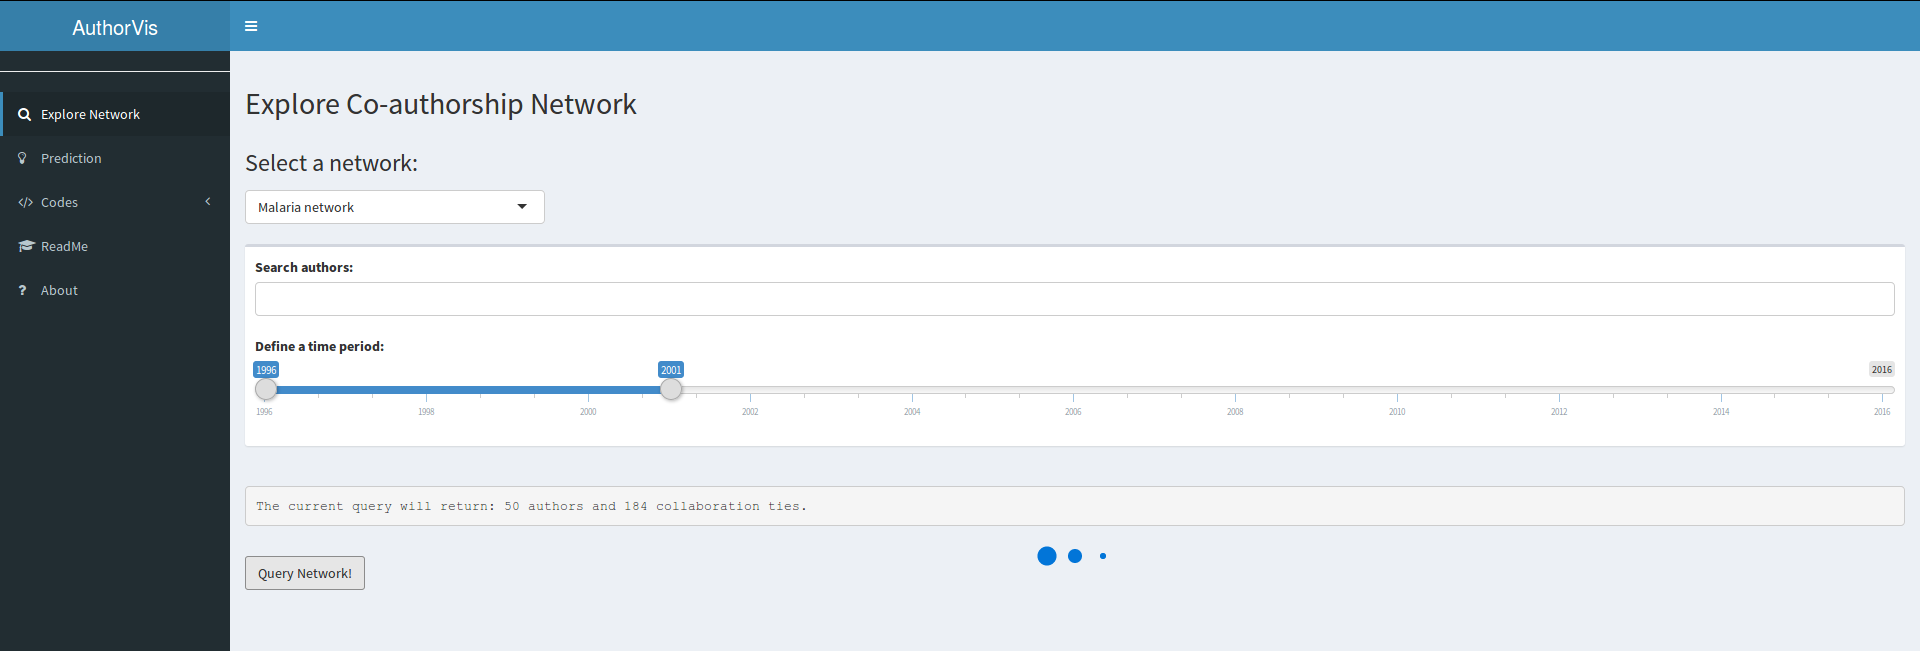
\includegraphics[scale=0.26]{Chapters/authorvis/screen2}
~\\~\\
\hspace{-1.5cm}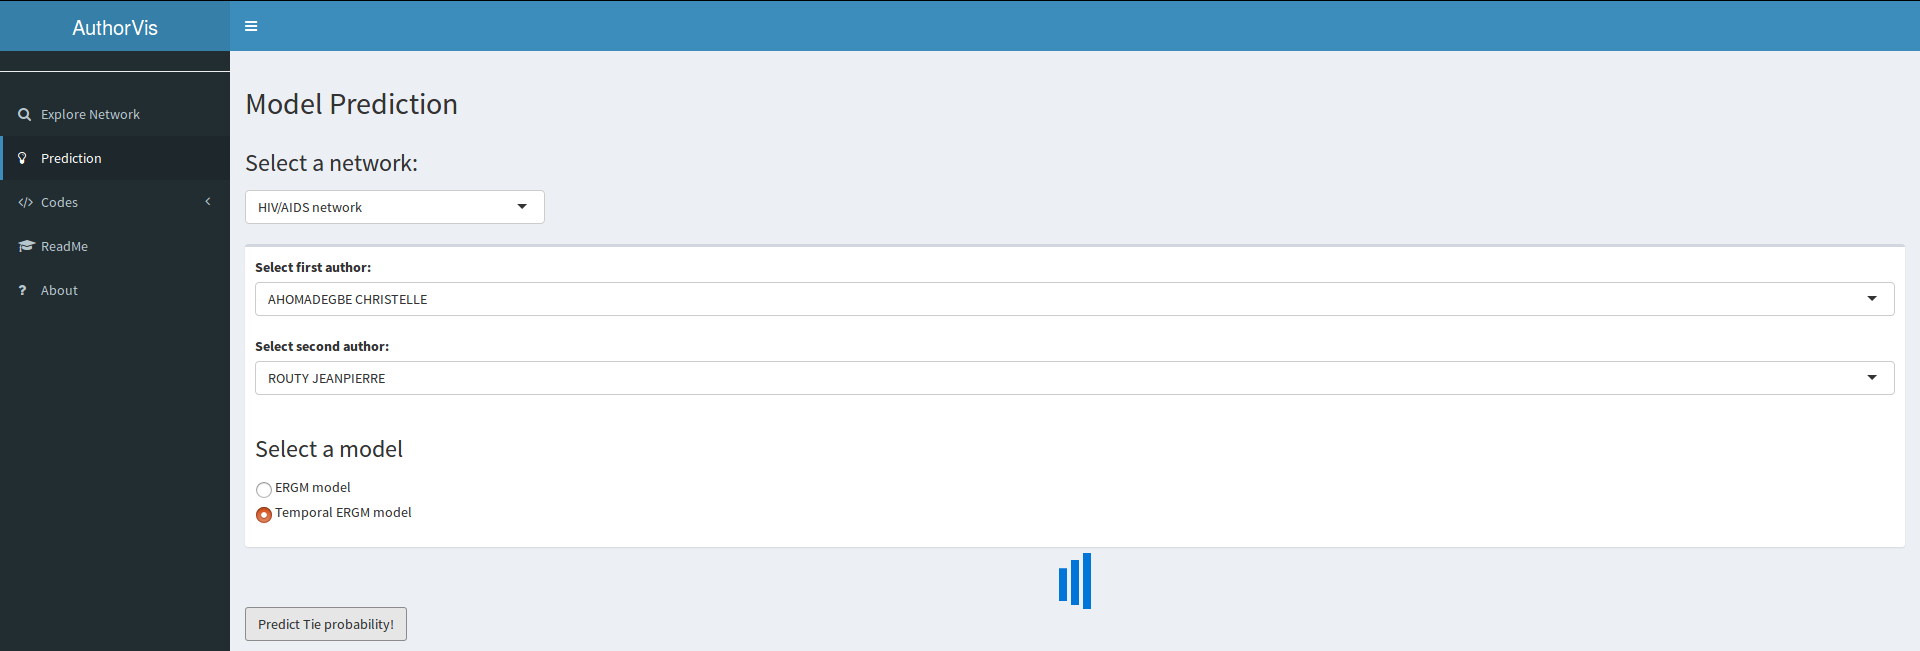
\includegraphics[scale=0.26]{Chapters/authorvis/screen4}
\caption{Screenshots of the Shiny application interface.}
\label{authorvis_screen1}
\end{figure}

\subsection{Data}
Currently, \textbf{AuthorVis} is designed specifically for the visualization of the Malaria, Tuberculosis and HIV/AIDS collaborative network in Benin. We refer the reader to section \ref{sec:data_collection} for details on the collection and treatment of the co-authorship data. On the server end, each network data is maintained as an igraph object. Each submitted user query is interpreted and incorporated in an igraph function to extract the network data. Another igraph object is generated as a result and converted into a JSON data using a specific Python script.

\subsection{Network Visualization}
The frontend network visualisation is built using the Javascript D3.js \cite{bostock_d3._2012}. We built in a navigation panel allowing the user to interact with the network and control physics of network \cite{newman_physics_2008}. We incorporated several Javascript functions to design an intuitive and user friendly visualization interface. A mouse hover over a vertex displays a tooltip of details on the author represented by the vertex while a double-click on a vertex highlights the subnetwork of the identified network. We made edges clickable. Once an edge is clicked, the list of published materials co-authored by the two vertices defining the clicked edge is displayed in a panel on the right hand side. All published materials listed can be traced back to their publication page on the web via their DOI or the WOS accession number with a single click.

\begin{figure}[!ht]
\centering
\hspace{-1.5cm}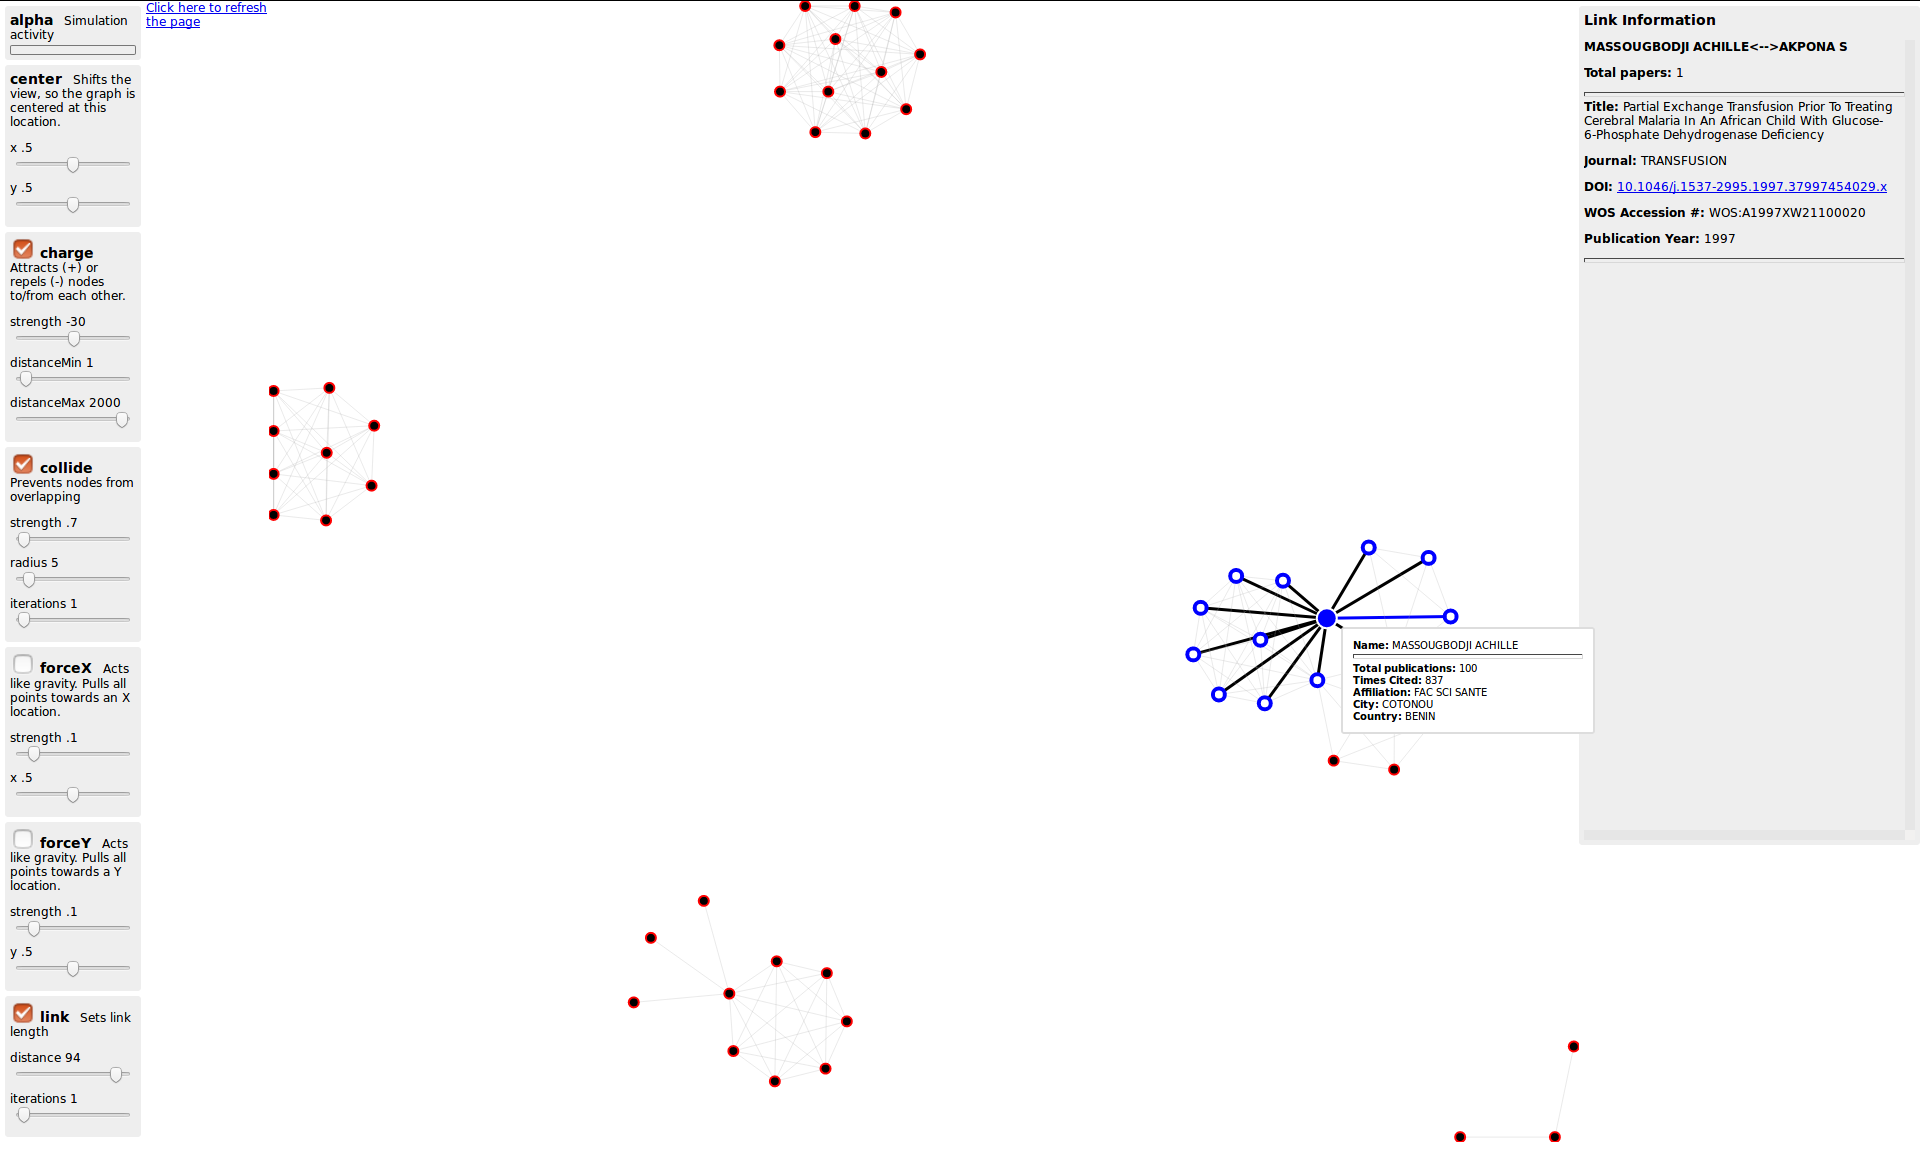
\includegraphics[scale=0.26]{Chapters/authorvis/vis3}
\caption{Screenshot of the co-authorship network visualization interface.}
\label{net_vis}
\end{figure}


\subsection{Web Framework}
The whole system is built into a Shiny dashboard thanks to the R package \textbf{Shinyboard} \cite{chang_shiny:_2017,chang_shinydashboard:_2015}. Using the dashboard, the user can choose to use the prediction tool menu, or query and visualize the network data. We also provide within the dashboard all our Shiny codes and a link to our Git directory containing all our source codes. \\
The prediction tool is model based and used the ERGM models to calculate a probability of collaboration between two authors. A micro-interpretation of the model is provided based on the user query  \cite{desmarais_micro-level_2012}. \\
When the user chooses the visualization menu, an interface allows him to submit his query to the system. The query is interpreted and processed on the server end and the user is automatically prompted to a new visualization page.

\section{Deployment}
The visualization front-end is maintained by an Python http-server. The system is packed in a Docker container to facilitate its use and installation. The project source files can be forked or cloned from Github at \url{https://github.com/rosericazondekon/authorvis}. We also made it accessible online via an  \href{https://#}{AWS server}.

%\section{Future Directions}
%Currently, \textbf{AuthorVis} is specifically built for Malaria, TB and HIV/AIDS in Benin. Future development will extend the tool to other research domain. We also aim at adding a general purpose module to \textbf{AuthorVis} for the visualization of any user-input co-authorship network. This will also require the integration of a data pre-processing module to facilitate the disambiguation and deduplication of co-authorship information. Finally, we will also incorporate a layered structured network visualization \cite{nakazono_nel_2006} functionality to the visualization in order to display temporal changes in the evolution of the co-authorship network.


%\section{Conclusion}
%Text for this section goes here...